\chapter{Case-study: A privacy-Preserving Video Doorbell}

This chapter presents a case study that focuses on the design and implementation of a specific type of IoT device - an Internet-enabled video doorbell. We assume the communication model to be the user-to-IoT model. The IoT device (video doorbell) is located in the user’s home network and communicates with the end-user device (smartphone).

\section{System design}
In addition to the security guarantee described in the last chapter, video doorbell systems have unique features. Here we present the design of the specific system.

\subsection{Use case analysis}
We consider there should be four prominent use cases in the system:
\begin{itemize}
	\item \textbf{Registration.} The user should be able to register a mobile device to the doorbell. Only trusted devices can access the data and manage settings.
	\item \textbf{Video streaming.} The user with a registered device should be able to access video captured by the camera at any time he wishes.
	\item \textbf{Face detection and push notification.} Whenever a visitor shows in front of the camera and/or pressed the physical doorbell button, all users registered to the doorbell should receive a push notification message.
	\item \textbf{Setting management.} The user should be able to manage settings, including changing face detection threshold, recording voice to be played, removing trusted devices, etc.
\end{itemize}

\textit{Fig. \ref{fig:usecase}} shows the use case diagram of the system.

\begin{figure}
	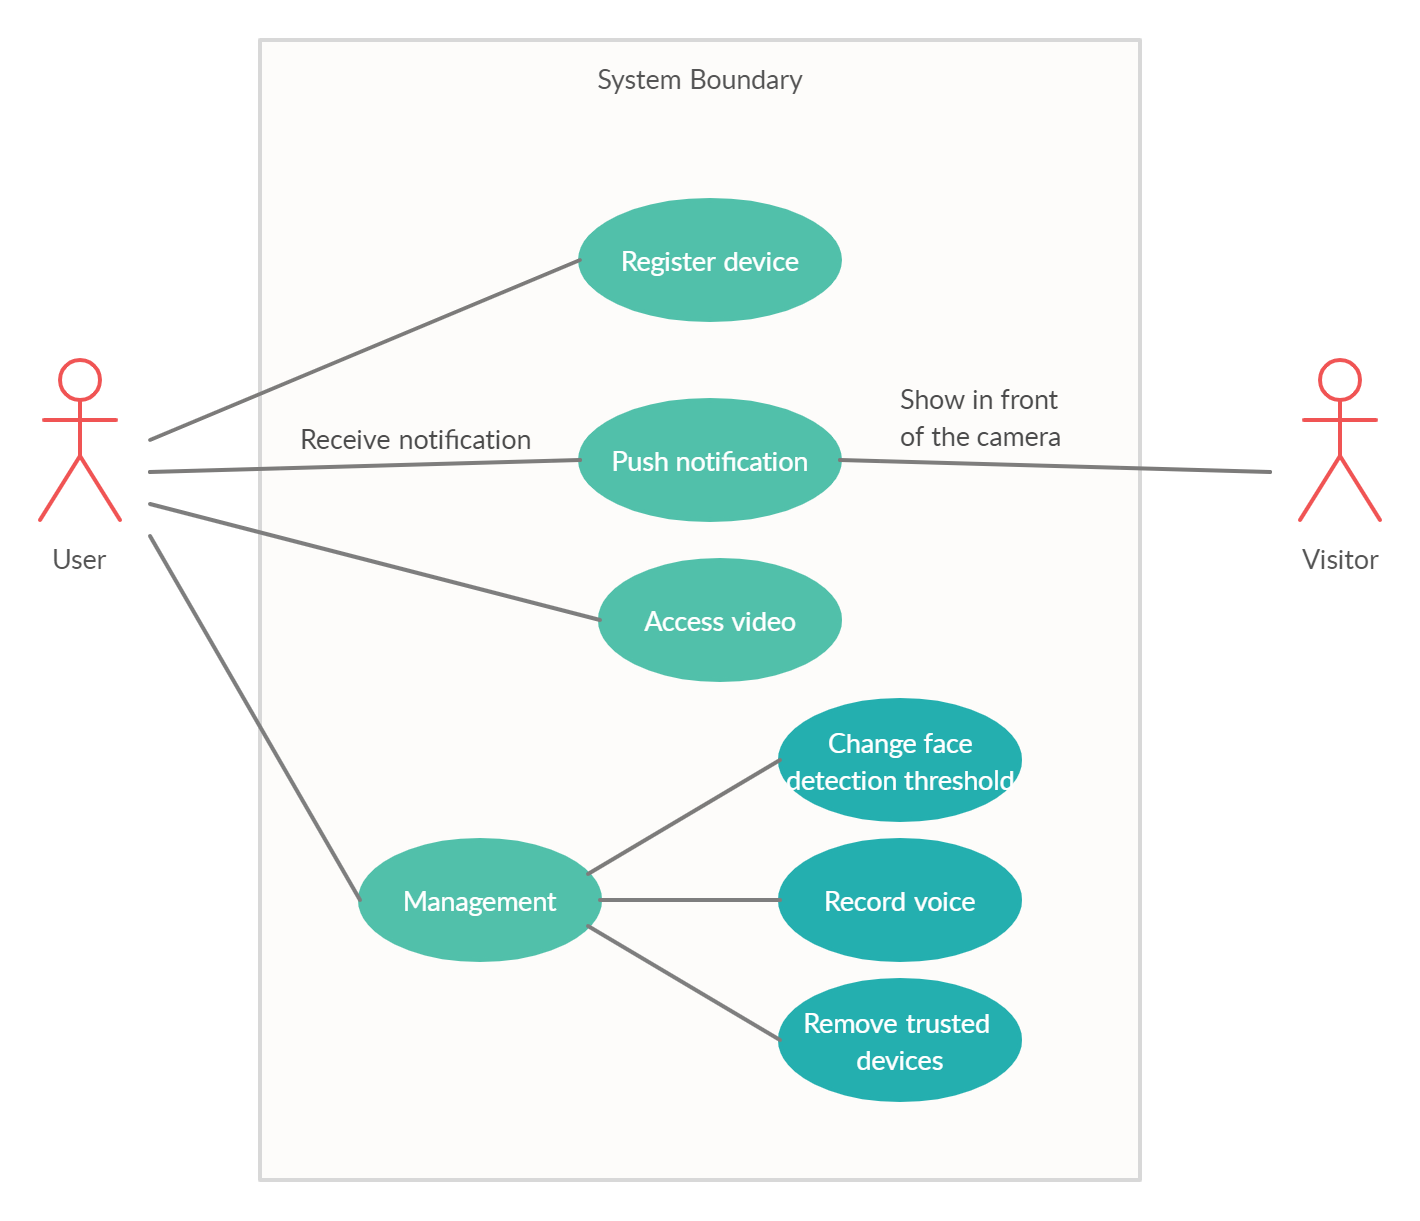
\includegraphics[width=\linewidth]{Use_case_diagram.png}
	\caption{}
	\label{fig:usecase}
\end{figure}

\subsection{Network architecture}
\textit{Fig. \ref{fig:architecture}} shows the network architecture of the system. Both the client and server are behind Tor for anonymity. Besides, we configure Tor on the doorbell side to use Snowflake \cite{snowflake} pluggable transport for obscuration.

\begin{figure}
	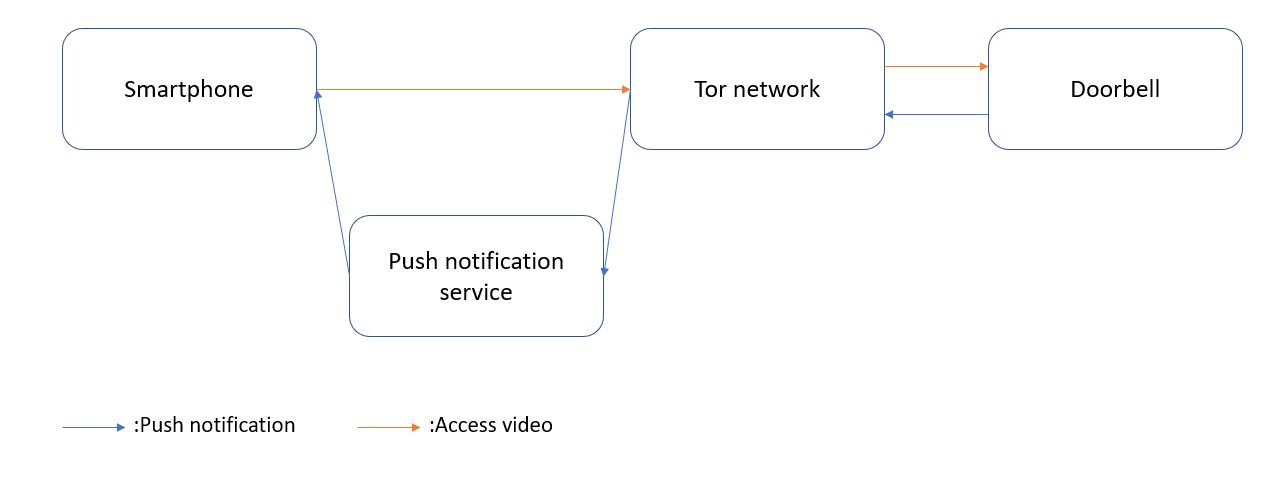
\includegraphics[width=\linewidth]{architecture.png}
	\caption{}
	\label{fig:architecture}
\end{figure}

\subsection{Flow structure}

\textbf{Registration.} The very first stage of using the system is the registration process. To have their devices registered on the doorbell, the users should first connect to the same wireless network with the doorbell. Then the app should allow the user to register (by searching the doorbell using mDNS) easily. During the registration process, the app performs a key exchange with the doorbell and receives randomly generated credentials for the user to set up in Tor (Orbot). 

\textbf{Playing video and authentication.} As soon as the user presses the PLAY button in the app, it will work with Orbot and send an RTMP PLAY request to the video server running on the doorbell. The video server will then forward an authentication request (in the form of an HTTP GET request) to the authentication server (running on another port on the doorbell). The server should serve video to the user through Tor if the authentication succeeds (i.e., the app is registered and has not been revoked) and shut down the connection otherwise.
\textit{Fig. \ref{fig:playvideo}} shows the flow of playing video and authentication.

\textbf{Face detection, push notification, and answering the door.} The doorbell constantly detects if there is a human face appearing in front of the camera. Whenever a visitor appears, the system should send a notification to the user's devices.

By clicking on the notification message on her phone, the user should be able to access the video immediately and choose to play pre-recorded audio on the doorbell device to the visitor.
\textit{Fig. \ref{fig:push}} shows the flow of face detection, push notification, and answering the door.

\begin{figure}
	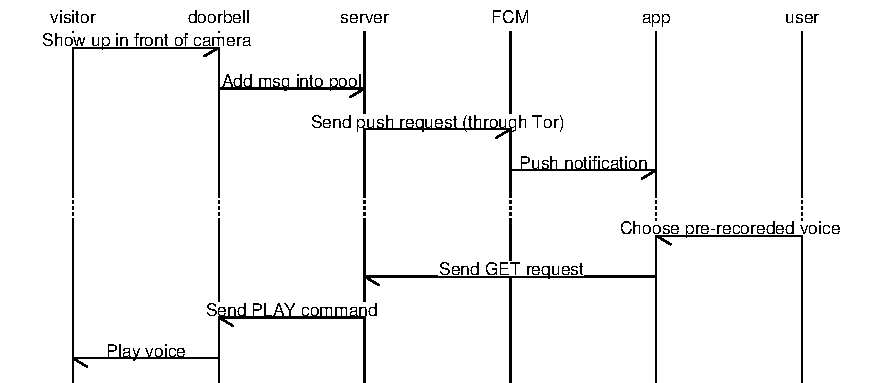
\includegraphics[width=\linewidth]{Sequence_diagram_push.pdf}
	\caption{}
	\label{fig:pushnotification}
\end{figure}
\begin{figure}
	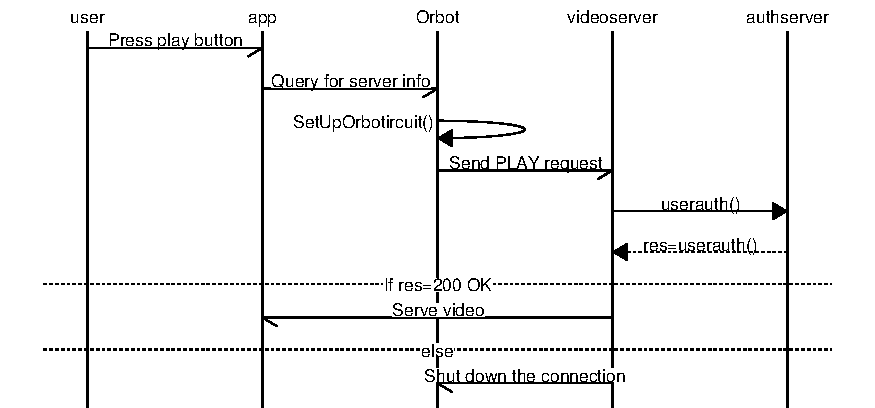
\includegraphics[width=\linewidth]{Sequence_diagram_playvideo.pdf}
	\caption{}
	\label{fig:playvideo}
\end{figure}
\begin{figure}
	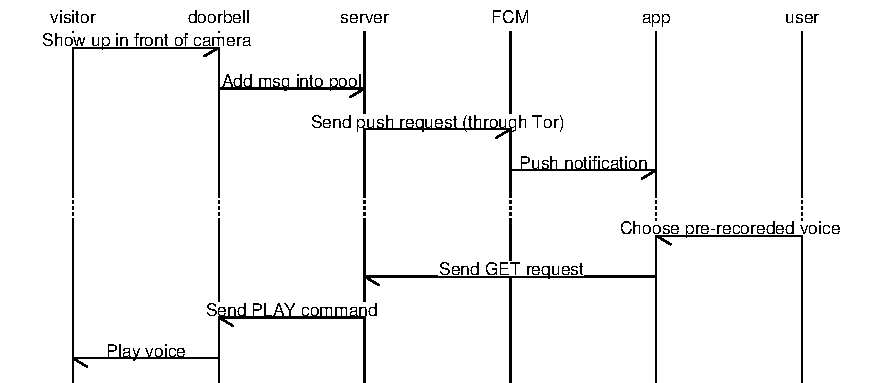
\includegraphics[width=\linewidth]{Sequence_diagram_push.pdf}
	\caption{}
	\label{fig:push}
\end{figure}

\section{Specs of the devices}
We configured a RaspberryPi 4 model B as the doorbell device. The RaspberryPi 4 has a built-in Wi-Fi antenna, and we combined the device with a camera module and external sound card. The RaspberryPi ran the Raspbian Jessie OS, which is a version of Debian Linux optimized for the RaspberryPi platform.

The RaspberryPi 4 model is equipped with more than 2GB of RAM and a CPU of 1.5 GHz, making it more than enough for a typical home IoT device.

\section{Face detection}

For the face detection task, we use the pre-trained CascadeClassifier. Cascade Classifiers based on Haar-like features were introduced in 2001 and are still widely used in face detection \cite{sharifara2014general}. Pre-trained Cascade Classifiers have a short execution time and small calculation load, making them a good choice for on-device calculations on IoT devices with low computational power.

We sample 6 frames per second in the actual implementation, transform them into gray-scale images, and feed them to the pre-trained classifiers. The detector is disabled for 5 seconds (which also matches the push notification interval) after a successful detection to prevent abusing resources. 

\section{Push notification}
To notify the user whenever a visitor is present in front of the camera, the system adapts Google's Firebase Messaging Service.

We designed two types of messages: \textbf{BELL} (sent when someone pushes the doorbell device’s physical button) and \textbf{DOOR} (sent when someone comes in front of the camera). The packet includes a message (including the type mentioned above), a timestamp, and the user's instance token. The message and timestamp are encrypted using AES-256-GCM with pre-shared keys (which are shared in the registration process described later).

In order to prevent the third-party service provider from obtaining information by analyzing the timing information, we further cover the traffic using another message type \textbf{DUMMY}, and send messages in a fixed interval of 5 seconds. The dummy packets have very similar structures to the normal ones, but have different types to be recognized by the client app. By padding the dummy packets to the traffic, the system sends a packet every 5 seconds.






\section{Video streaming}
The doorbell device captures video using the RaspberryPi's camera module and audio through an external sound card. The video captured is encoded and served in flv format through HTTP. We chose to decode the videos in flv format because it is consistent among different operating systems and suitable for future enhancement of support on other platforms. 

Our system adopts two layers of authentication on top of video streaming. The first layer of authentication is \textit{onion authentication}. Provided along with Tor, it requires the user to have specific credentials set up in their Tor (Orbot) client. The onion host refuses to connect if one does not have such settings or has different settings. The second layer of authentication is the \textit{RTMP authentication}. In order to access the video, the user will have to add a couple of arguments in addition to their RTMP PLAY request. \textit{Fig. \ref{fig:url}} shows the components of the video serving URL. In the URL, \textit{appname} and \textit{streamname} are Nginx settings and of the user's choice. \textit{usertoken} is a random number securely generated from the client app (upon the first launch), and the following equation calculates userpassword:

\[
userpassword = HMAC-SHA256(seed, usertoken)
\]

The server checks if \textit{all} credentials match and shut down the connection if any are incorrect.

\begin{figure}
	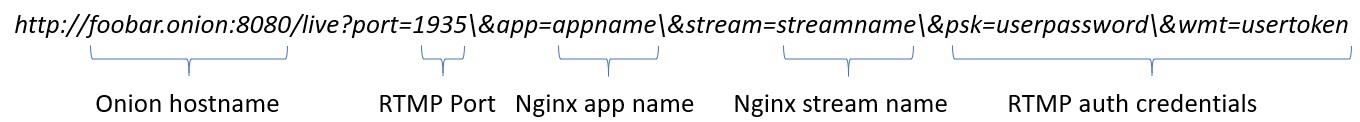
\includegraphics[width=\linewidth]{fig_url.jpg}
	\caption{}
	\label{fig:url}
\end{figure}



\section{Android App}
We implemented an Android App to pair with the video doorbell service. The app runs on the end-user device and grants users direct access to the doorbell device and data. The app has the following primary functions:

\subsection{Registration} For registration, the client sends JSON-formatted data in an HTTP POST request to port 8080 of the server (running on the doorbell device). The server will then respond with another JSON-formatted data, including the seed (randomly generated 16-bit integer) for calculating the secret keys, the onion hostname for accessing the video service, and the onion authentication cookie. The app will then automatically send a configuration string (including the authentication cookie) required by Orbot to the user’s clipboard for her to set up the service quickly. 

\textit{Fig. \ref{fig:app_sc_main}} shows the main (registration) GUI of the app.


\subsection{Media player} The app has the VLC player integrated for video streaming. Working with Orbot, the media player plays the video through the Tor network, which prevents adversaries from eavesdrop into the transmitted video.

\subsection{Management} The client sets up a webpage for the user to manipulate settings, including changing detection threshold, revoking authentications, recording voice, etc. The management page is only accessible in the local network (that saying, the user device must be in the same wireless network with the doorbell device to manipulate settings) and requires a password for access.

\textit{Fig. \ref{fig:app_sc_management}} shows the preference page, and \textit{Fig. \ref{fig:app_sc_token_revoke}} shows the token management (where user can revoke trusted devices) of the app.

\begin{figure}
	\begin{minipage}[t]{0.3\linewidth}
		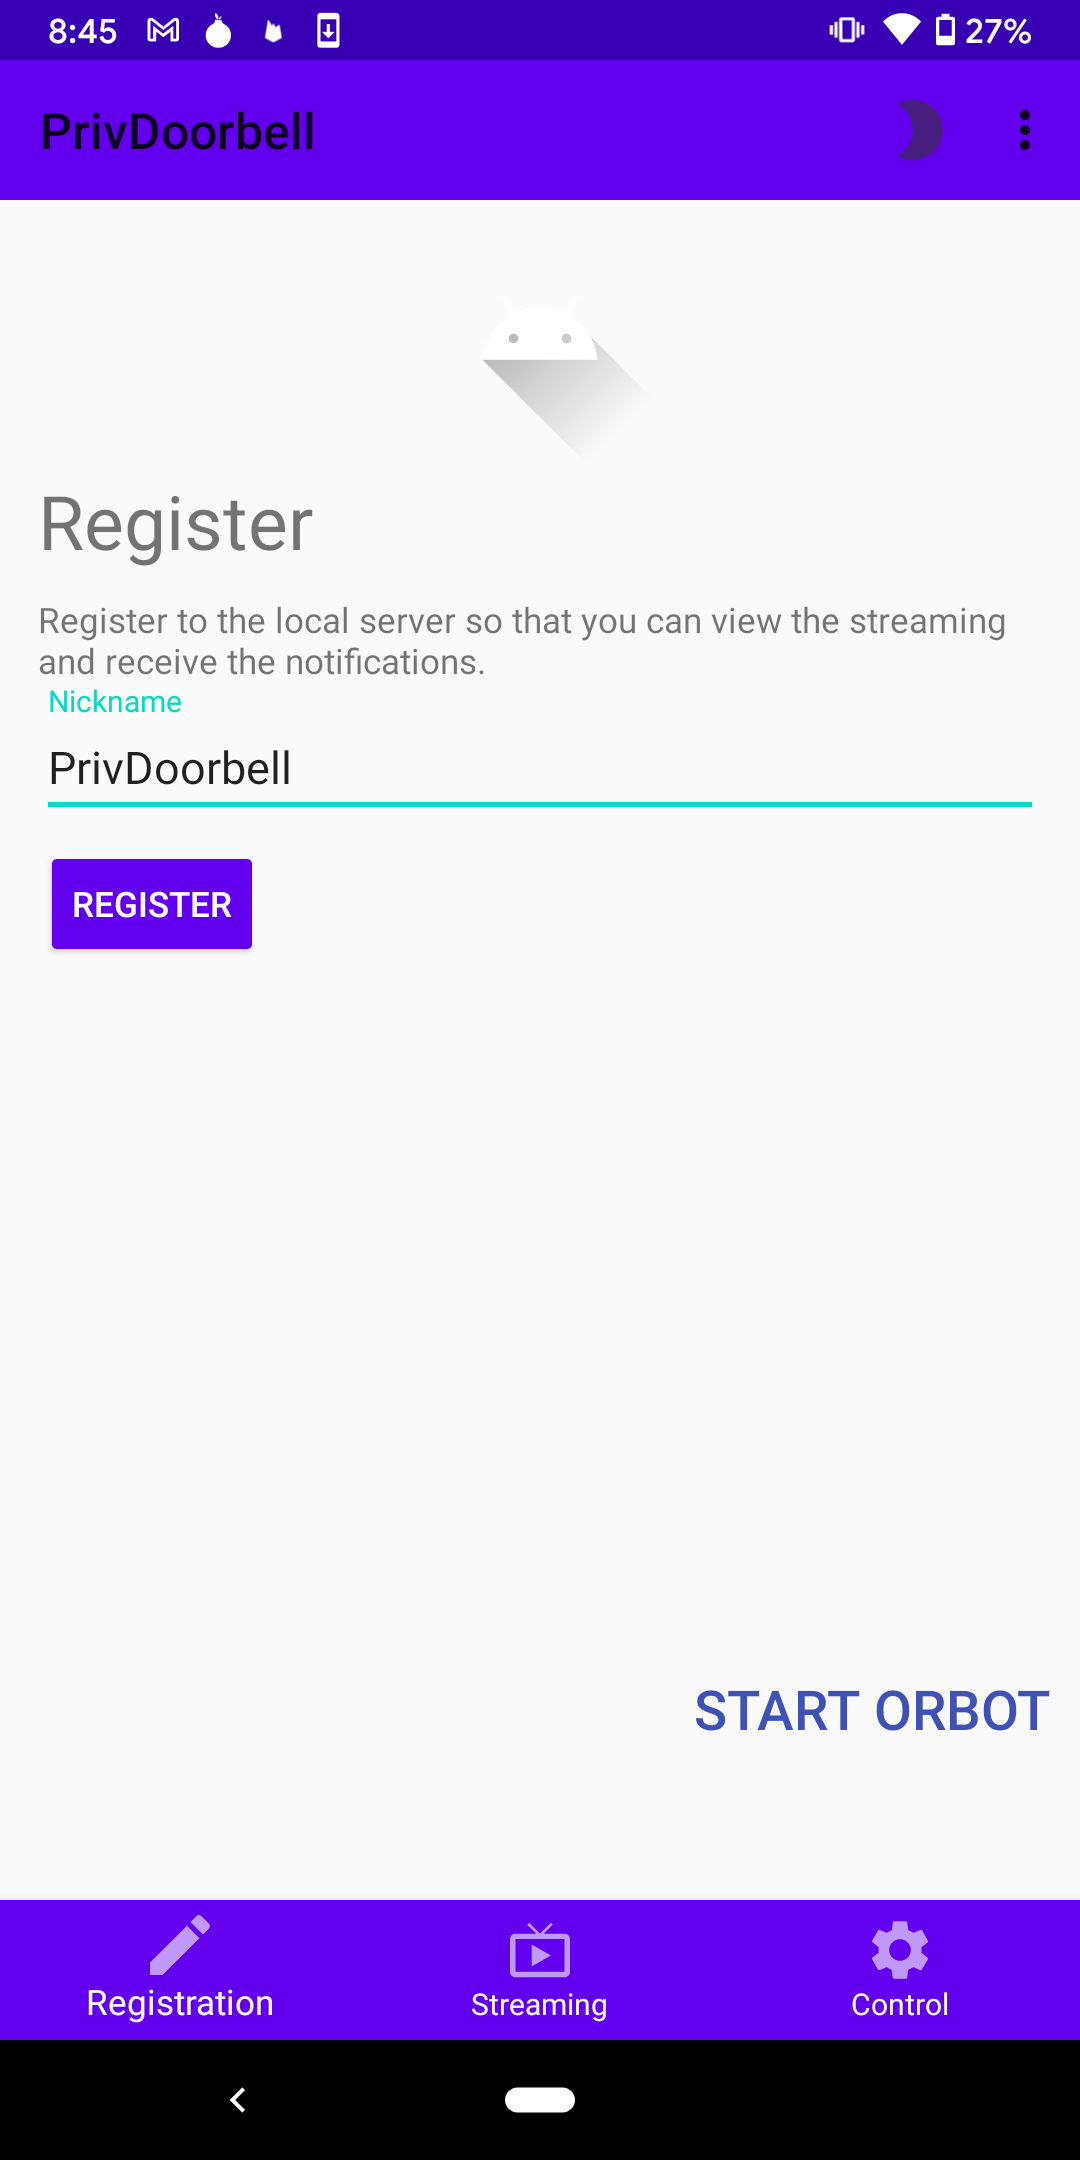
\includegraphics[width=0.5\linewidth]{app_sc_main.png}
		\caption{}
		\label{fig:app_sc_main}	
	\end{minipage}
	\begin{minipage}[t]{0.3\linewidth}
		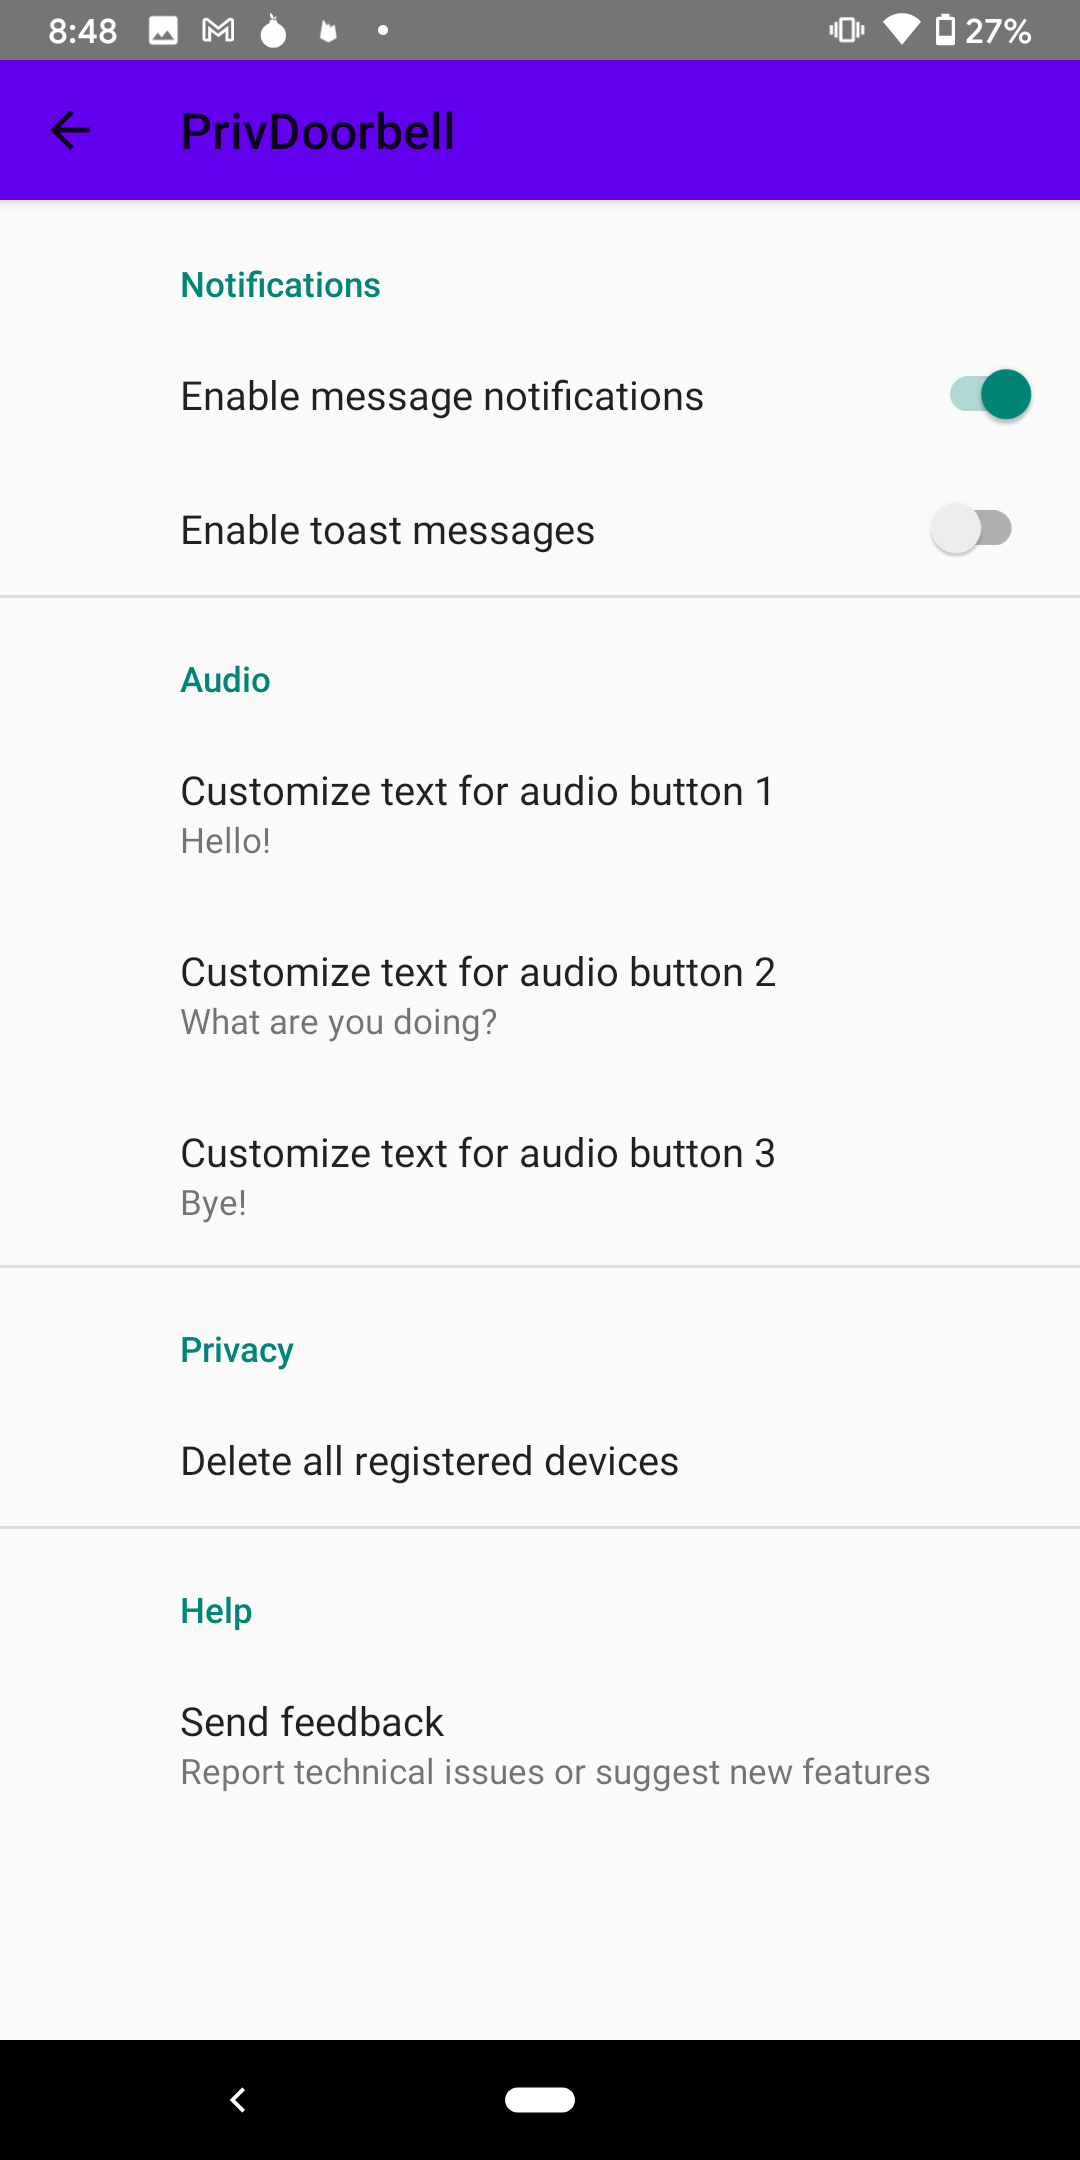
\includegraphics[width=0.5\linewidth]{app_sc_management.png}
		\caption{}
		\label{fig:app_sc_management}
	\end{minipage}
	\begin{minipage}[t]{0.3\linewidth}
		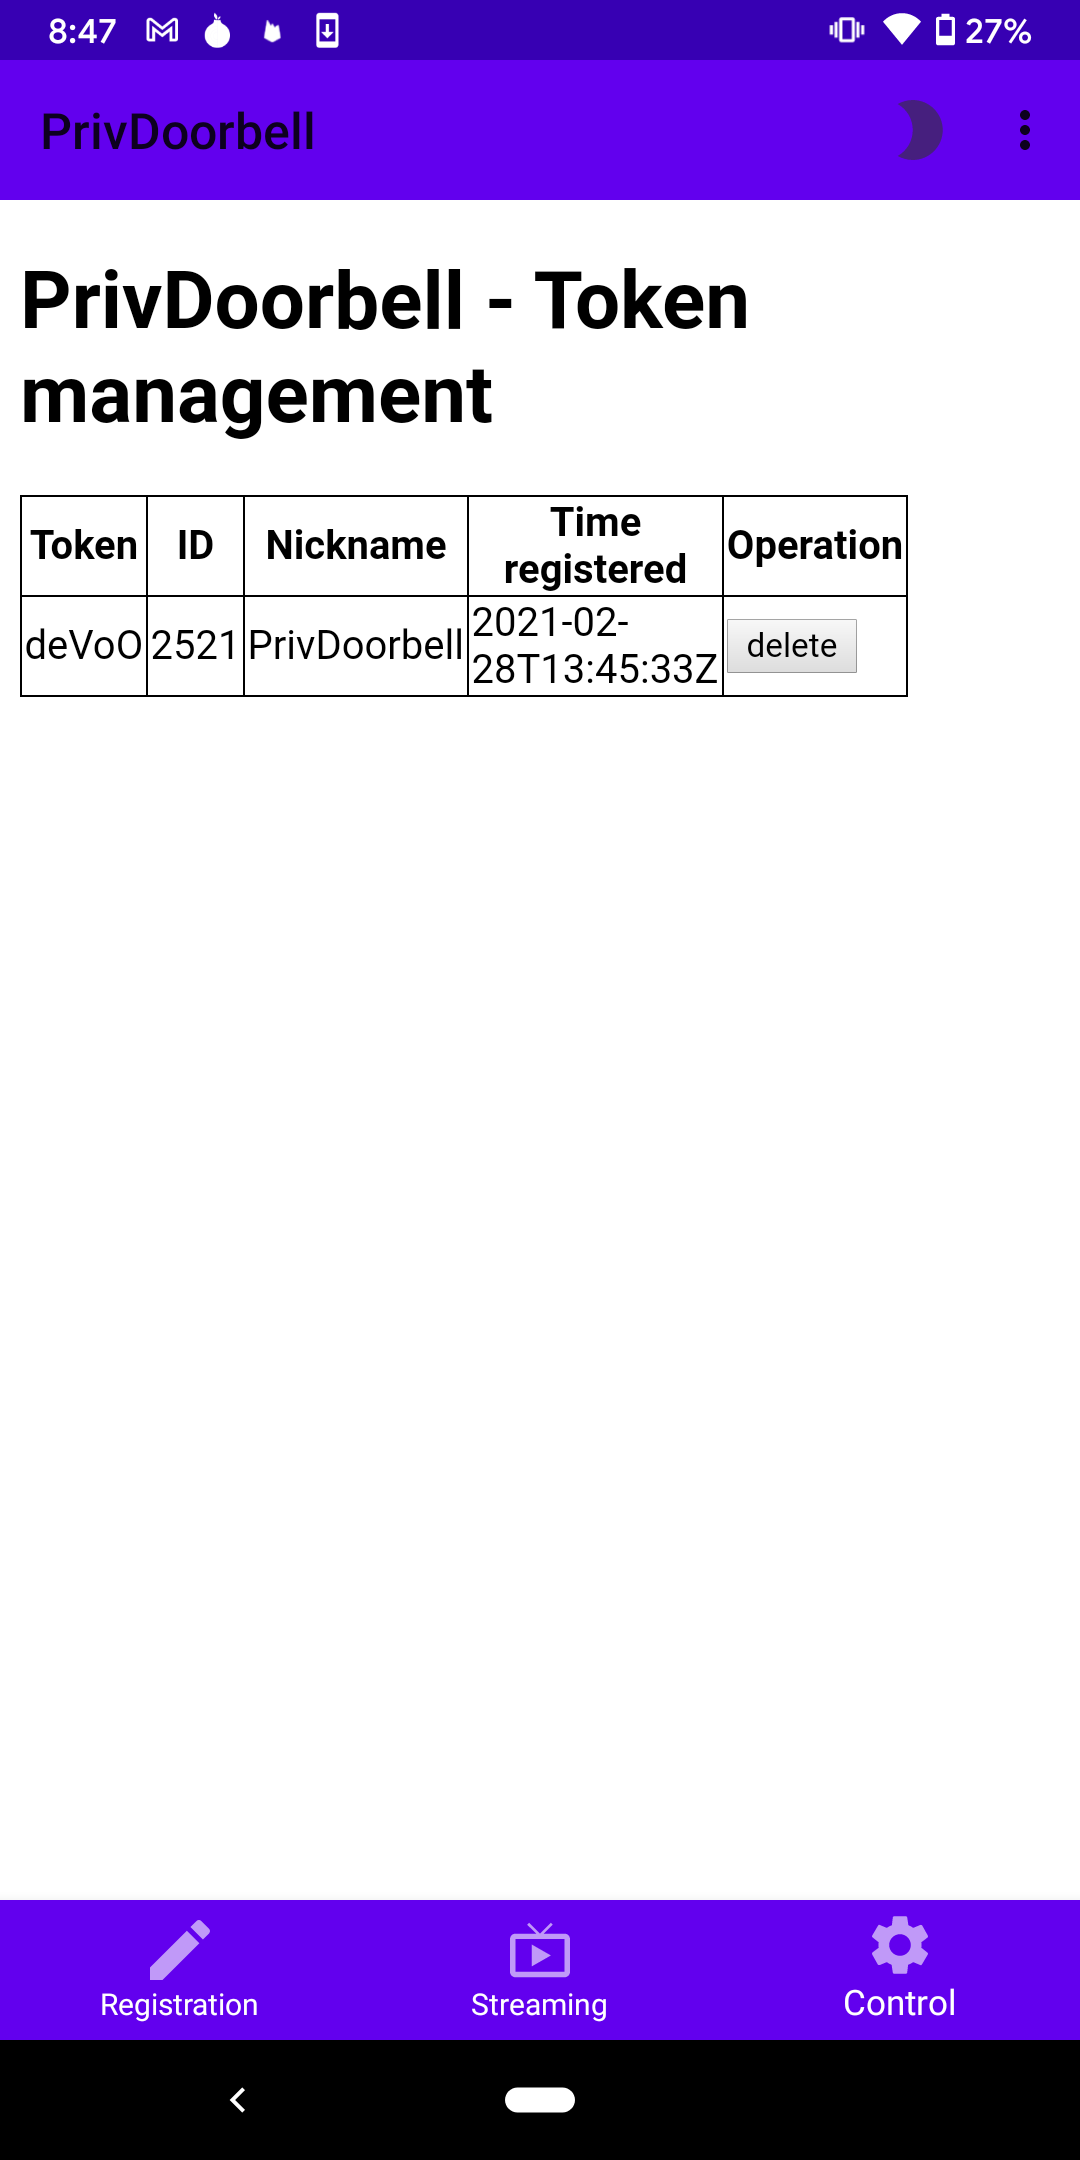
\includegraphics[width=0.5\linewidth]{app_sc_token_revoke.png}
		\caption{}
		\label{fig:app_sc_token_revoke}
	\end{minipage}	
\end{figure}


\section{Experimental study}
In this section, we would like to evaluate the performance of our system by analyzing the following factors:
\begin{itemize}
	\item Streaming latency
	\item Energy consumption
	\item Bandwidth
	\item Notification latency
	\item The cost of using Tor
\end{itemize}

A Google Pixel 3a XL is used as the client device.

\subsection{Streaming latency}
\label{subsec:streaming_latency}
We measure our system's latency as the time difference between the user’s pressing on the Play button and the first frame’s appearing. \textit{Fig. \ref{fig:timeconsumption}} shows the time taken for 100 samples. We divide the time into four phrases.
\begin{itemize}
	\item Circuit: The \textit{Circuit} phrase is from when the app starts processing the user’s request to when it receives the server's information. In this phrase, the app queries the proxy (Orbot) about the onion URL. Orbot will then try to establish a circuit connection between the user device and the server. In practice, the time taken in this phrase varies, as sometimes there is an existing circuit. If Tor has to create a new circuit, this phrase typically takes a few more seconds. On average, this phrase takes 2.355 seconds with a standard derivation of 3.07 seconds.
	\item Transmission: The \textit{Transmission} phrase is from when the app sends request to the server to when the app hears back from the server. As we are using RTMP authentication, the server should return a HTTP answer code 200 if the client provides correct credentials. The video transmission will begin immediately after the HTTP response. In average, this phrase takes 0.599 seconds with a standard derivation of 0.089 seconds.
	\item Preparation: The \textit{Preparation} phrase is from when the app receives HTTP answer from the server to when it starts filling the buffer. In this phrase, the media player initializes its components and gets ready for playing the video. In average, this phrase takes 3.878 seconds with a standard derivation of 0.715 seconds.
	\item Buffering: The \textit{Buffering} phrase is when the app fills in its buffer. In this phrase, the media player fill a few frames into the buffer (of a programmed size) for the decoder to decode. The decoder will do the work in milliseconds, and thus we can consider the video being played immediately after this phrase. In average, this phrase takes 0.046 seconds with a standard derivation of 0.006 seconds.
\end{itemize}

\begin{figure}
	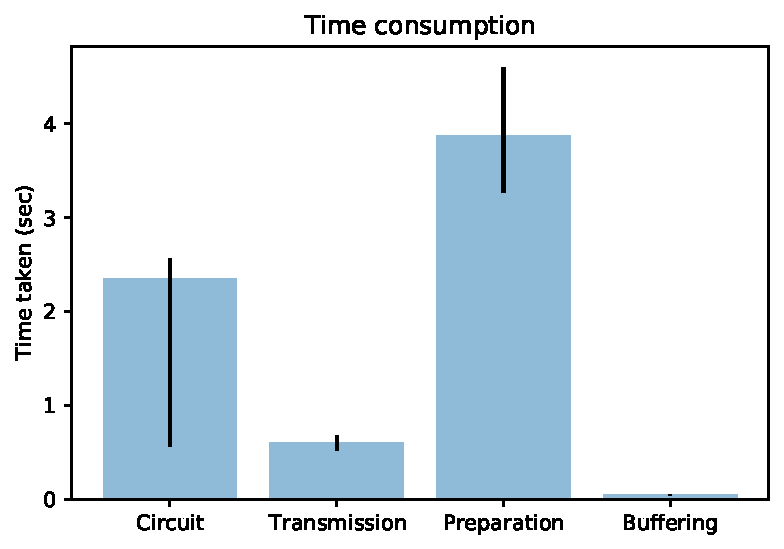
\includegraphics[width=\linewidth]{plot1.pdf}
	\caption{}
	\label{fig:timeconsumption}
\end{figure}

\begin{figure}
	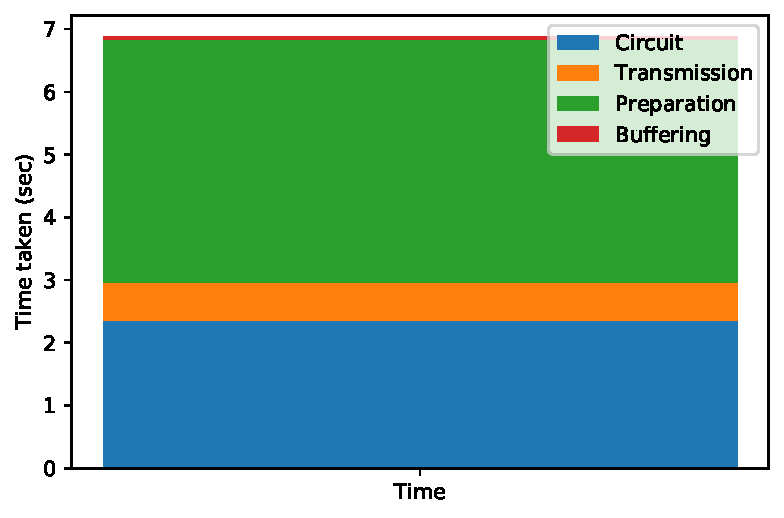
\includegraphics[width=\linewidth]{plot2.pdf}
	\caption{}
	\label{fig:timepercentage}
\end{figure}

In average, the whole process takes 6.867 seconds with a standard derivation of 3.141 seconds. \textit{Fig. \ref{fig:timepercentage}} shows how much time each phrase takes.


\subsection{Energy consumption}
We evaluate the battery consumption of our app using the system measured data. The app consumes 6\% of the device's battery after actively running in background for 6 days, 11 hours and 50 minutes (83.83 hours). The device has a battery size of 3700 mAh, and therefore the app roughly consumes 2.65 mAh for every hour running. We consider it reasonable for an app which receives and pushes real-time notifications.

\subsection{Bandwidth}
The outgoing traffic from the doorbell devices is 71 kb/s by average, after the video is compressed and encoded. For comparison, the raw video has the size of 410 kb/s.

\subsection{Video and audio quality}
The system supports videos up to 1024x768/6fps and audio with sample rate of 44.1kHz.

\subsection{Notification latency}
\label{subsec:notification_latency}
We measure the notification latency by measuring the time difference from when the message is sent to Firebase Messaging server from the doorbell to when the message is received on the client app. The average latency of 250 consecutive samples is 0.478 second. Fig. \cite{fig:notificationlatency_wTor} shows the CDF (cumulative distribution function) vs. latency (in second) diagram.

\subsection{The cost of using Tor}
Finally, we would like to measure the cost of using Tor. By its nature, Tor adds latency to the system and we would like to know the exact impact. We measure the following time and compare the difference:

\begin{itemize}
	\item Streaming latency
	\item Notification latency
\end{itemize}

\begin{figure}
	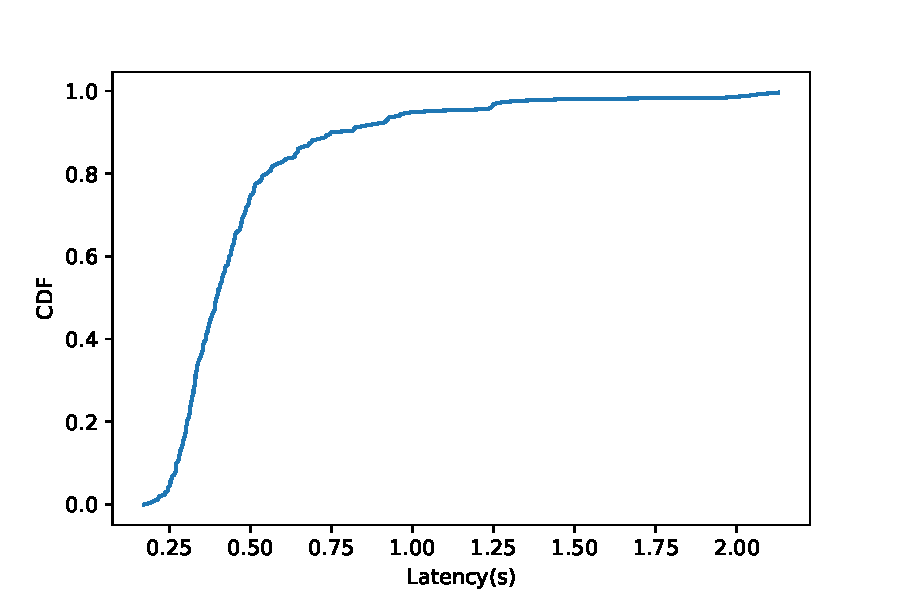
\includegraphics[width=\linewidth]{notification_latency_withTor.pdf}
	\caption{}
	\label{fig:notificationlatency_wTor}
\end{figure}

\paragraph{Streaming latency} 

We described the streaming latency of our system in \ref{subsec:streaming_latency}. For a simple comparison, launching the streaming takes 2.240 second on average.

\paragraph{Notification latency}

As we described in \ref{subsec:notification_latency}, the latency of push notification with Tor is 0.478 second on average. We further conduct experiment where Tor is not in the middle. \textit{Fig. \ref{fig:notificationlatency_wTor_vs_vanilla}} shows the difference of the service with Tor ("with-Tor") between that without Tor ("vanilla"). The dotted green line stands for the latency of vanilla service, and the blue full line stands for the latency of with-Tor service. The median of with-Tor service is roughly twice as the median of vanilla service.

\begin{figure}
	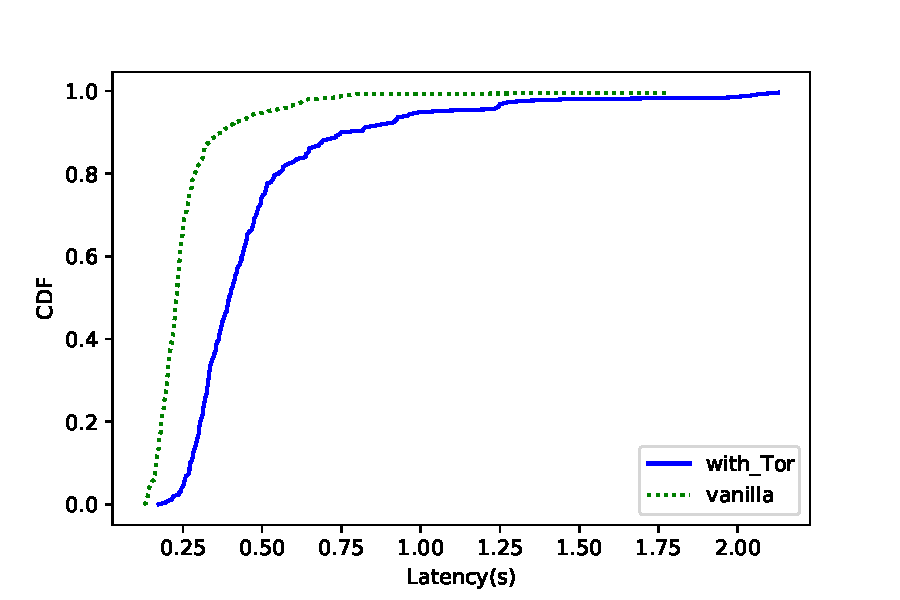
\includegraphics[width=\linewidth]{plot_push_tor_vs_vanilla.pdf}
	\caption{}
	\label{fig:notificationlatency_wTor_vs_vanilla}
\end{figure}